\section{Карта теорем и навигация по доказательствам}
\label{sec:oc13-theorem-roadmap}

Эта глава представляет собой наиболее ясную и компактную карту доказательного маршрута. Её задача — показать, где проходит опорный скелет теорем, какие классы утверждений несут какую научную нагрузку и какие участки следует в первую очередь проверять враждебному рецензенту. Она не заменяет формальные главы и руководство по чтению. Руководство по чтению отвечает за пути входа; эта глава — за навигацию в доказательстве.

\subsection{Опорный скелет теорем}

На уровне обоснования bounded journal-core текущий релиз опирается на относительно небольшой опорный скелет, хотя сама монография существенно объёмнее. Схема ниже является компактной, а не минимальной в строгом теоретико-доказательном смысле: в ней оставлена заметной ветвь остаток--возрождение, поскольку защищаемая theorem-уровневая теорема классифицирует post-collapse идентичность, а не только смерть. Поэтому скелет можно задавать в виде схемы зависимостей, а не объектно-языкового импликационного правила. Чтобы маршрут не выглядел как исчисление доказательств, карта опоры записана как помеченные review-edges:

\begin{enumerate}
\item \textbf{Ребро 1.} Axiom~3.2 вместе с Definitions~12.1, 12.3 и 12.4 поддерживает Source Theorem~3, а Source Theorem~3 поддерживает Lemma~1.
\item \textbf{Ребро 2.} Axiom~3.3 вместе с Definition~12.6 поддерживает Source Corollary~3.2, а Source Corollary~3.2 поддерживает Lemma~3.
\item \textbf{Ребро 3.} Lemma~1 вместе с Definition~12.5 поддерживает Lemma~2.
\item \textbf{Ребро 4.} Lemma~2 является единственной посылкой, зафиксированной для Theorem~A в canonical proof-obligation registry.
\end{enumerate}

В этом перечне определения играют роль узлов-предпосылок, а не самостоятельных теоремных посылок. Слово ``supports'' обозначает принятый шаг поддержки релиза, а не примитивный оператор импликации OC.

В этой дорожной карте Lemma~3 остаётся принятый обязанностью по контролю возрождения, но не является посылкой Theorem~A в canonical proof-obligation registry. Её нагрузочная роль иная: оно поддерживает сопутствующее контрольное утверждение, Proposition~B. Когда сжатое доказательство статьи обсуждает блок death--residue--rebirth в одном абзаце, Lemma~3 следует читать как поддерживающее Proposition~B, в то время как Theorem~A остаётся классификацией death-and-residue через Lemma~2.

\paragraph{Proposition B (article-local rebirth control).}
\label{prop:oc13-rebirth-control}
В рамках article-level-извлечения после того, как \(K\) надлежащим образом схлопнулся так, что \(\Omega(K)=\emptyset\) и \(k(K,t)=0\), более поздний объект \(K'\) классифицируется как возрождение тогда и только тогда, когда \(K'\) жив, численно отличается от исходного мёртвого контура \(K\), находится либо в той же ветви вложения, либо в явно подтверждённой связанной ветви вложения, наследует хотя бы один объявленный элемент резидуальной опоры и удовлетворяет соответствующим условиям рождения. Правило тождества объясняет, почему условие неидентичности здесь обязательно, а не факультативно. Это утверждение — сопутствующее контрольное для ветви возрождения; оно не является посылкой Theorem~A.

В этой roadmap приставка \emph{Source} обозначает свидетельскую проекцию из аудируемого публичного корпуса LaTeX-исходников и архивного скомпилированного PDF, описанного в приложении source-audit. Такие строки переносятся в Core~1.3 как источником подтверждённые узлы поддержки и рассматриваются через canonical proof-obligation registry; они не являются новыми примитивными теоремами article-level-извлечения. Немаркированные леммы, Theorem~A и Proposition~B представляют собой производные строки article-level, собранные из этой источниковой поддержки. Theorem~A использует скелет death-and-residue; Proposition~B использует ветвь rebirth-control.

Аксиоматические утверждения, теоремы и следствия источника, леммы и Theorem~A несут proof-force-узлы; определения фиксируют термины, используемые в этих узлах.

Смысл явного построения этой цепочки не в том, чтобы выдавать, будто вся рамка сводится к одной диаграмме. Цель — показать, что ограниченное утверждение имеет проверяемое позитивное ядро, а не сводится к облаку мотивационной прозы. Рисунок~\ref{fig:oc13-theorem-spine} также отмечает один исключённый lift-heavy маршрут как грань враждебного рецензирования; он рассматривается именно для того, чтобы его нельзя было спутать с принятой поддержкой в позитивной цепочке. Ветвь Corollary~3.2 / Lemma~3 показана как принятая ветвь rebirth-control для Proposition~B рядом с теоремным маршрутом, а не как предпосылка Theorem~A. В этой roadmap ветвь related-embedding представлена одним проверяемым article-level-свидетелем, а не исчерпывающим перечнем всех допустимых source-level-свидетелей related-embedding. Это та же ветвь, обозначаемая \(\mathcal{M}\sim_{\mathrm{res}}\mathcal{M}'\) в Section~\ref{sec:oc13-worked-examples}: именованное структуросохраняющее отображение \(h:\mathcal{M}\to\mathcal{M}'\), резидуальный элемент \(r\in R_{\mathrm{res}}(K)\), принадлежность к допустимой области \(h(r)\in\Omega(K')\subseteq\Omega_{\mathrm{amb}}(\mathcal{M}')\) и сохранение пороговых и допустимых предикатов на резидуально-насыщенной подструктуре. Section~\ref{sec:oc13-worked-examples} и journal core явно формулируют это тестирование свидетеля.

\begin{figure}[htbp]
\centering
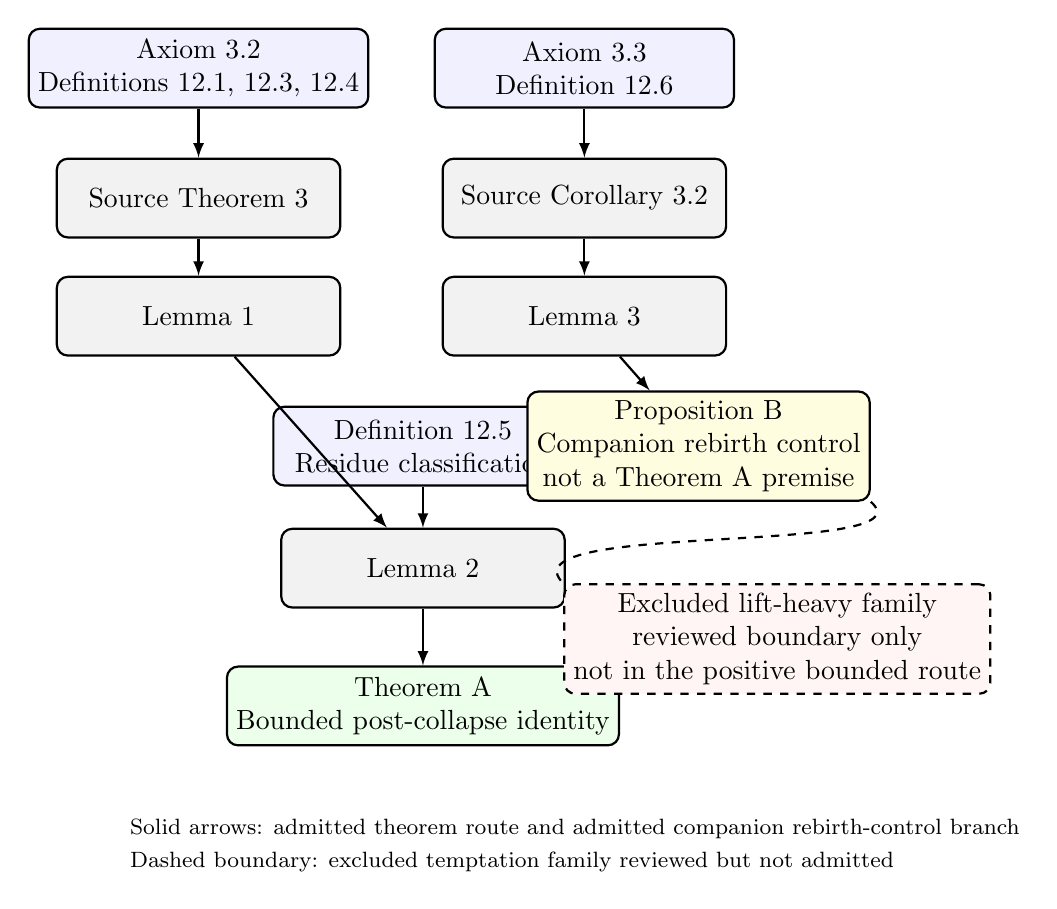
\begin{tikzpicture}[
    >=latex,
    thick,
    node distance=1.45cm and 0.8cm,
    proofnode/.style={draw, rounded corners, fill=gray!10, align=center, minimum width=3.6cm, minimum height=1.0cm},
    supportnode/.style={draw, rounded corners, fill=blue!6, align=center, minimum width=3.8cm, minimum height=1.0cm},
    excludednode/.style={draw, rounded corners, dashed, fill=red!4, align=center, minimum width=3.8cm, minimum height=1.0cm},
]

\node[supportnode] (leftsupport) at (0, 3.2) {Axiom 3.2\\Definitions 12.1, 12.3, 12.4};
\node[proofnode] (sourcethm) at (0, 1.55) {Source Theorem 3};
\node[proofnode] (lemmaone) at (0, 0.05) {Lemma 1};

\node[supportnode] (rightsupport) at (4.9, 3.2) {Axiom 3.3\\Definition 12.6};
\node[proofnode] (sourcecor) at (4.9, 1.55) {Source Corollary 3.2};
\node[proofnode] (lemmathree) at (4.9, 0.05) {Lemma 3};

\node[supportnode] (defresidue) at (2.85, -1.6) {Definition 12.5\\Residue classification};
\node[proofnode] (lemmatwo) at (2.85, -3.15) {Lemma 2};
\node[proofnode, fill=green!8, minimum width=4.1cm] (theorema) at (2.85, -4.9) {Theorem A\\Bounded post-collapse identity};

\node[proofnode, fill=yellow!12, minimum width=4.1cm] (propositionb) at (6.35, -1.6) {Proposition B\\Companion rebirth control\\not a Theorem A premise};
\node[excludednode] (excludedlift) at (7.35, -4.05) {Excluded lift-heavy family\\reviewed boundary only\\not in the positive bounded route};

\draw[->] (leftsupport) -- (sourcethm);
\draw[->] (sourcethm) -- (lemmaone);
\draw[->] (rightsupport) -- (sourcecor);
\draw[->] (sourcecor) -- (lemmathree);
\draw[->] (lemmaone) -- (lemmatwo);
\draw[->] (defresidue) -- (lemmatwo);
\draw[->] (lemmatwo) -- (theorema);
\draw[->] (lemmathree) -- (propositionb);

\draw[dashed] (propositionb.south east) .. controls +(0.8,-0.7) and +(-0.8,0.8) .. (excludedlift.north west);

\node[anchor=north west, align=left] at (-1.0, -6.2) {\footnotesize Solid arrows: admitted theorem route and admitted companion rebirth-control branch\\\footnotesize Dashed boundary: excluded temptation family reviewed but not admitted};

\end{tikzpicture}

\caption{Опорный скелет теорем ограниченного утверждения Core~1.3. Сплошные стрелки обозначают принятую поддержку. Позитивный путь Theorem~A заканчивается на Lemma~2; ветвь Lemma~3 остаётся видимой как принятая поддержка rebirth-control рядом с этим путём. Пунктирная ветвь обозначает исключённый lift-heavy маршрут, рассматриваемый как граничное условие рецензирования, а не как включённый элемент позитивного доказательства. Более объёмная монография остаётся необходимой, потому что окружающие главы задают онтологию, операторный каркас, доктрину уровней K, грамматику коллапса, эмпирический порог и аудит-слои, благодаря чему этот скелет остаётся научно интерпретируемым и внешне цитируемым.}
\label{fig:oc13-theorem-spine}
\end{figure}

\subsection{Что окружает скелет}

У опорного скелета теорем небольшой объём доказательной зависимости, но он интерпретируется и контролируется внутри более широкого корпуса рукописи по пяти направлениям:

\begin{enumerate}
\item формальные главы доктрины фиксируют admissibility, пороги, операторы, уровни, ветвление и опровержимость;
\item главы consistency и source-boundary фиксируют класс утверждений, судьбу теорем и рамки публикации;
\item глава proof-machinery и приложение фиксируют revision, comparator, compression и дисциплину proof-obligation;
\item главы operational и empirical фиксируют promotion, replay и дисциплину falsifier;
\item приложения удерживают аудитную нагрузку и атлас внутри того же тома.
\end{enumerate}

Поэтому монография может быть больше defended article, не становясь риторически размытою. Окружающие главы — это publication- и audit-среда, а не дополнительные посылки Theorem~A.

\subsection{Классы утверждений и нагрузка}

Таблица ниже — это карта proof-navigation для рецензента. Она следует таксономии классов утверждений из Section~\ref{sec:oc13-foundational-consistency}. Строка proposition — это только навигационное подразделение производных утверждений, а не новый класс proof-status. Operational rules остаются последующей нагрузкой контроля, а не отдельным class proof-status.

\begin{table}[htbp]
\centering
\begingroup
\footnotesize
\RaggedRight
\setlength{\tabcolsep}{4pt}
\begin{tabular}{@{}L{0.21\textwidth}L{0.28\textwidth}L{0.39\textwidth}@{}}
\toprule
\textbf{Класс утверждений} & \textbf{Научная нагрузка} & \textbf{Где проверять} \\
\midrule
Аксоматические утверждения & Фиксируют примитивные условия admissibility, идентичности или порогов. & Appendices Axioms, Appendices Notation и Sections~\ref{sec:boundary-extended}--\ref{sec:collapse-rebirth}. \\
Производные теоремы и леммы & Несут основное доказательное позитивное тело. & Sections~\ref{sec:results}, \ref{sec:collapse-rebirth}, \ref{sec:oc13-theorem-roadmap}, Reviewer Navigation Matrix и Proof Machinery Appendix. \\
Утверждения article-level & Несут сопутствующие контрольные утверждения, выведенные из той же аудируемой опоры, но не являющиеся посылками Theorem~A. Примером является Proposition~B (rebirth-control). & Sections~\ref{sec:oc13-theorem-roadmap}, \ref{sec:oc13-worked-examples} и Journal Core Bridge Appendix. \\
Структурные утверждения & Объясняют иерархию, структуру модулей и связи между уровнями или артефактами. & Sections~\ref{sec:klevels-full}--\ref{sec:falsifiability-extended}, Section~\ref{sec:modules_master}, Section~\ref{sec:oc13-publication-boundary} и Section~\ref{sec:oc13-foundational-consistency}. \\
Интерпретирующие утверждения & Объясняют смысл, неформальные акценты и последующие границы. & Sections~\ref{sec:discussion}, \ref{sec:oc13-worked-examples}, \ref{sec:oc-core-1-3-practical-utility}, Source Audit Appendix и Reviewer Navigation Matrix. \\
Эмпирические утверждения & Требуют source-owned domain packet, theorem-native trace, численного закона параметров, наблюдаемой фиксации, закреплённого маршрута данных, held-out replay, аудита comparator и falsifier перед promotion. & Sections~\ref{sec:oc-core-1-3-operationalization-program}--\ref{sec:oc-core-1-3-empirical-execution-protocols} и Appendices~\ref{sec:oc-core-1-3-empirical-validation-matrix}--\ref{sec:oc-core-1-3-domain-execution-board}. \\
Фронтирные утверждения & Отмечают допустимое продолжение работы в будущем без права позитивного релиза. & Section~\ref{sec:oc-core-1-3-practical-utility}, Appendix~\ref{sec:oc-core-1-3-practical-utility-atlas} и frontier-строки в source-owned science corpus. \\
\bottomrule
\end{tabular}
\endgroup
\caption{Классы утверждений и их нагрузка проверки в Core~1.3. Таблица не заменяет формальные главы; она лишь предотвращает перемещение ролей между доказательством, интерпретацией, эмпирическим promotion и frontier-языком. Replay, comparator, falsifier и escalation rules — это последующие контрольные обязанности, прикреплённые к этим классам.}
\label{tab:oc13-statement-classes}
\end{table}

Все цели проверки в Table~\ref{tab:oc13-statement-classes} сверяются по меткам с английским мастер-источником. Если release-оболочка меняет одну из этих меток, таблицу нужно регенерировать или откорректировать прежде, чем roadmap будет считаться механически воспроизводимым маршрутом аудита.

\subsection{Самый короткий hostile-review checklist}

Если рецензент хочет наиболее эффективную последовательность проверки, наиболее логически сложные проверки остаются следующими:

\begin{enumerate}
\item проверьте, что коллапс действительно связан с потерей допустимой реализации, а не с свободной метафорой;
\item проверьте, что правило необратимости запрещает восстановление исходного континуума как численно тождественной сущности;
\item проверьте, что residue и rebirth выступают управляемыми классификациями, а не повествовательными ярлыками;
\item проверьте, что исключённая семья lift-heavy теорем не подмешана обратно в bounded позитивный маршрут;
\item проверьте, что journal-core-извлечение не утверждает ничего более сильного, чем source-owned science corpus и canonical SPOT-разрешение; тогда флагманская монография проверяется только как производная сравнительная поверхность;
\item проверьте, что доктрина уровней K, в особенности \(K_{11}\) и \(K_{12}\), обоснована структурно, а не раздута риторически.
\end{enumerate}

Если на этом этапе релиз терпит неудачу, более поздняя проза его не спасёт. Если он проходит этот этап, более медленное полное прочтение становится оправданным.

\paragraph{Переход к следующей главе.}
После построения карты доказательного маршрута следующая глава сознательно меняет режим. Она перестаёт абстрактно навигировать по скелету и показывает, как формальную грамматику следует читать через worked examples, counterexamples и bounded проверочные интерпретации.

\clearpage
